\graphicspath{ {./Figure/Figure11/}}
\begin{figure}
  \centering
	

  \hspace*{\fill}
  \subfigure[]{\label{subfig:9a}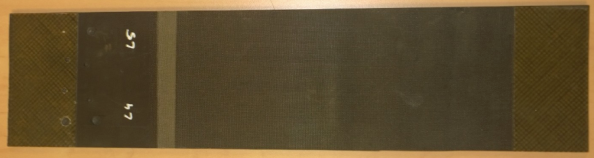
\includegraphics[width=0.3\linewidth]{fig9a.png}}
  \hspace*{\fill} \\ \hspace*{\fill}
  \subfigure[]{\label{subfig:9b}
\includegraphics[width=0.3\linewidth]{fig9b.png}} \hfill
  \subfigure[]{\label{subfig:9c}
\includegraphics[width=0.3\linewidth]{fig9c.png}} \hfill
  \subfigure[]{\label{subfig:9d}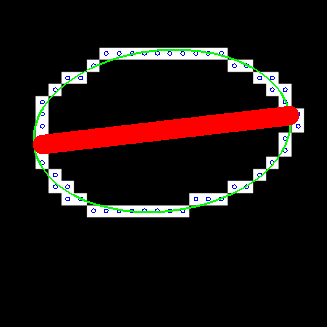
\includegraphics[width=0.3\linewidth]{fig9d.png}}
  \hspace*{\fill}
	  
		\caption{(a) The specimen - (b) Segmented thermal response - (c) Edge of the thermal
		response - (d) Ellipse fitting.}
		\label{fig:9}
		\end{figure}
